\subsection{Dealing with Asynchrony}

\begin{frame}[fragile]
    \frametitle{Attempt 1 - No Synchronization}
    \begin{algorithm}[H]
        \begin{algorithmic}[0]
            \STATE \textbf{operation} $REG[i].write(v)$ \textbf{is}
            \bindent
                \STATE $Reg[i].value \leftarrow v$
                \STATE $brodcast$ $WRITE(v)$
            \eindent

            \STATE \textbf{operation} $REG[j].read()$ \textbf{is}
            \bindent
                \STATE $return$ $Reg[j].value$
            \eindent
            
            \STATE \textbf{when a message} $WRITE(v)$ \textbf{arrives} from $p_j$ \textbf{do}
            \bindent
                \STATE $Reg[j].value \leftarrow v$
            \eindent

        \end{algorithmic}
        \caption{Incorrect algorithm with no synchronization}
        \label{alg:seq}
    \end{algorithm}
\end{frame}

\begin{frame}
    \frametitle{Algorithm 1 - Not even eventually consistent}
    \begin{center}
        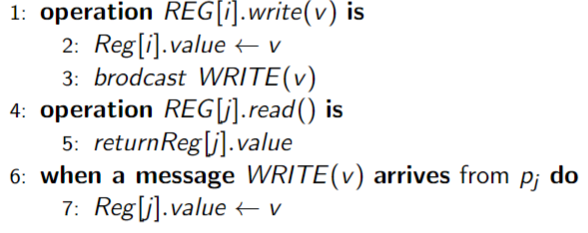
\includegraphics[scale=.7]{resources/alg1_src.png}
        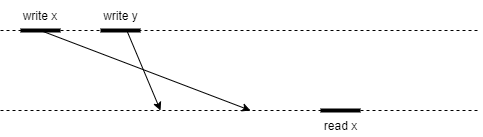
\includegraphics[scale=.5]{resources/alg1_incorrectness.png}
    \end{center}
\end{frame}

\begin{frame}[fragile]
    \frametitle{Attempt 2 - Write Synchronization}
    \begin{algorithm}[H]
        \begin{algorithmic}[0]
            \STATE \textbf{operation} $REG[i].write(v)$ \textbf{is}
            \bindent
                \STATE $sn\leftarrow sn+1$
                \STATE $Reg[i].value \leftarrow v$
                \STATE $brodcast$ $WRITE(v)$
                \STATE $\textbf{wait}$ $got$ $WRITE\_DONE(sn)$ $from$ $all$
            \eindent

            \STATE \textbf{operation} $REG[j].read()$ \textbf{is}
            \bindent
                \STATE $return$ $Reg[j].value$
            \eindent
            
            \STATE \textbf{when a message} $WRITE(v, sn)$ \textbf{arrives} from $p_j$ \textbf{do}
            \bindent
                \STATE $Reg[j].value \leftarrow v$
                \STATE $send$ $WRITE\_DONE(sn)$ $to$ $p_j$
            \eindent

        \end{algorithmic}
        \caption{wait on writes - Sequentially Consistent, but not Linerarizable}
        \label{alg:seq}
    \end{algorithm}
\end{frame}

\begin{frame}
    \frametitle{Algorithm 2 - Not Linearizable due to Read Inversion}
    \begin{center}
        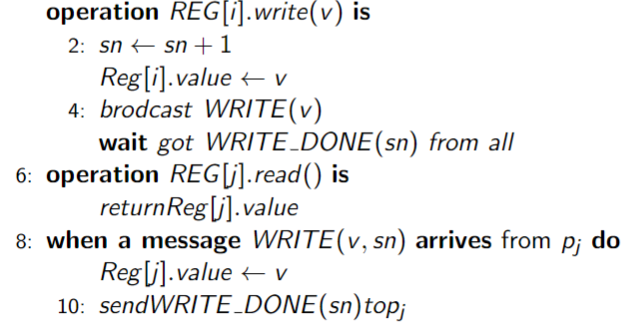
\includegraphics[scale=.63]{resources/alg2_src.png}
        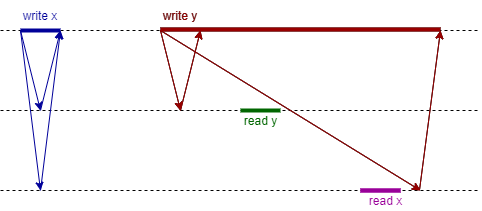
\includegraphics[scale=.5]{resources/alg2_incorrectness.png}
    \end{center}
\end{frame}

\subsection{Dealing with Write Inversion}
\begin{frame}[fragile]
    \frametitle{Attempt 3 - Waiting Read}
    \begin{algorithm}[H]
        \begin{algorithmic}[0]
            \STATE \textbf{operation} $REG[i].write(v)$ \textbf{is}
            \bindent
                \STATE $wsn\leftarrow wsn+1$
                \STATE $Reg[i].value \leftarrow v$
                \STATE $brodcast$ $WRITE(v)$
                \STATE $\textbf{wait}$ $got$ $WRITE\_DONE(wsn)$ $from$ $all$
            \eindent
        \end{algorithmic}
        \caption{Wait on both reads and writes -
            Linearizable but cannot handle faulty processes}
    \end{algorithm}
\end{frame}

\begin{frame}[fragile]
    \frametitle{Attempt 3 - Waiting Read. Cont.}
    \begin{algorithm}[H]
        \begin{algorithmic}[0]
            \STATE \textbf{operation} $REG[j].read()$ \textbf{is}
            \bindent
                \STATE $rsn[j]\leftarrow rsn[j]+1$
                \STATE $brodcast$ $READ(j, rsn[j])$
                \STATE $\textbf{wait}$ $got$ $STATE(wsn_k[j], rsn[j])$ $from$ $each$ $p_k$
                \STATE $sn := max\{rsn_k[j]\mid k\in[n]\}$
                \STATE $\textbf{wait}$ $rsn[j] \geq sn$
                \STATE $when$ $done:$ $w, sn \leftarrow Reg[j]$
                % \STATE $brodcast$ $CATCH\_UP(j, sn)$
                % \STATE $\textbf{wait}$ $got$ $CATCH\_UP\_DONE(j, sn)$ $from$ $all$
                \STATE $return$ $w$
                % why not just return Reg[j].value when done?
            \eindent
        \end{algorithmic}
        \caption*{}
    \end{algorithm}
\end{frame}

\begin{frame}[fragile]
    \frametitle{Attempt 3 - Waiting Read. Cont.}
    \begin{algorithm}[H]
        \begin{algorithmic}[0]
        \STATE \textbf{when a message} $WRITE(v, sn)$ \textbf{arrives} from $p_j$ \textbf{do}
        \bindent
            \STATE $Reg[j].value \leftarrow v$
            \STATE $send$ $WRITE\_DONE(sn)$ $to$ $p_j$
        \eindent
        \STATE \textbf{when a message} $READ(j, rsn)$ \textbf{arrives} from $p_j$ \textbf{do}
        \bindent
            \STATE $send$ $STATE(Reg[j].sn, rsn)$ $to$ $p_j$
        \eindent
        
        % \STATE \textbf{when a message} $CATCH\_UP(j, sn)$ \textbf{arrives} from $p_j$ \textbf{do}
        % \bindent
        %     \STATE $\textbf{wait}$ $Reg[j].sn \geq sn$
        %     \STATE $send$ $CATCH\_UP\_DONE(sn, rsn)$ $to$ $p_j$
        % \eindent
    \end{algorithmic}
        \caption*{}
    \end{algorithm}
\end{frame}

\begin{frame}
    \frametitle{Algorithm 3 - Cannot handle faulty processes}
    \begin{alertblock}{Faulty Processes?}
        \begin{itemize}
            \item $p_i$ writes, and waits for $WRITE\_DONE$ from $p_j$.
            \item $p_j$ fails.
            \item $p_i$ is stuck.
        \end{itemize}
    \end{alertblock}
    \begin{block}{Never wait for everyone!}
        What if we just wait for majority?\\
        If we don't change anything else, it will bring back read inversion.
    \end{block}
\end{frame}

\subsection{BAMP Algorithm}

\begin{frame}
    \frametitle{Algorithm 4 - BAMP}
    \begin{block}{Main Idea}
        Use the messages from \textbf{alg. 3} to provide linearizability,
        and use \textbf{majority} and \textbf{reliable brodcast}
        to handle faulty (including byzantine) processes.
    \end{block}
\end{frame}

\begin{frame}
    \frametitle{Initialization and Invocations}
    \begin{center}
        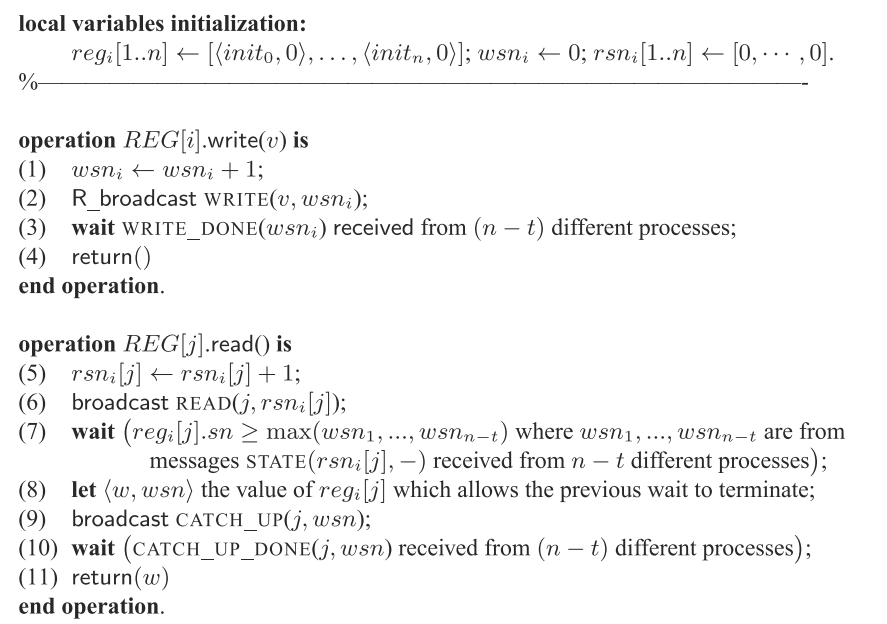
\includegraphics[scale=.7]{resources/alg4_src1.png}
    \end{center}
\end{frame}
\begin{frame}
    \frametitle{Message Handling}
    \begin{center}
        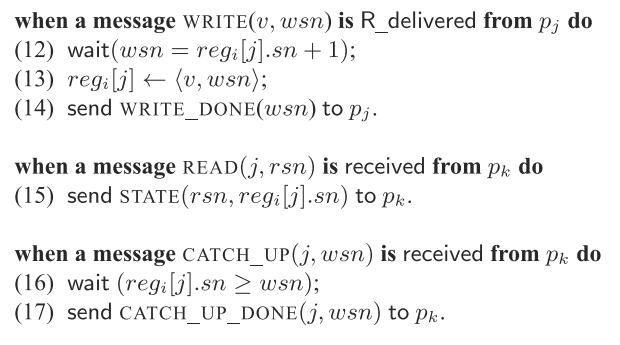
\includegraphics[scale=.7]{resources/alg4_src2.png}
    \end{center}
\end{frame}


\begin{frame}
    \frametitle{Algorithm 4 - No Read Inversion}
    \begin{center}
        \begin{figure}
            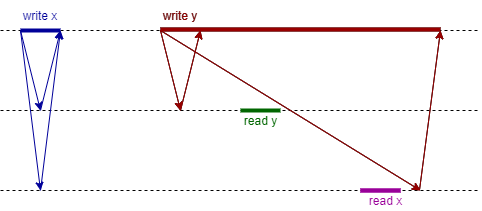
\includegraphics[scale=.35]{resources/alg2_incorrectness.png}
            \caption*{No Read Wait (alg. 2).}
        \end{figure}
        \begin{figure}
            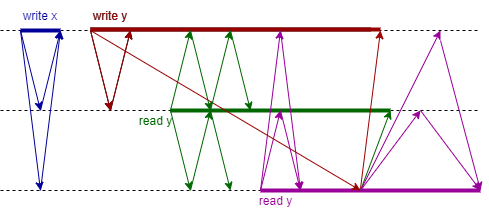
\includegraphics[scale=.35]{resources/alg3_no_read_inversion.png}
            \caption*{With Read Wait (alg. 3).}
        \end{figure}
    \end{center}
\end{frame}